\documentclass[12pt,onecolumn,a4paper]{article}
\usepackage{float}
\usepackage{epsfig,graphicx,subfigure,amsthm,amsmath}
\usepackage{color,xcolor}     
\usepackage{xepersian}
\usepackage{graphicx}

\settextfont[Scale=1.2]{BZAR.TTF}
\setlatintextfont[Scale=1]{Times New Roman}


\begin{document}
\newpage
\tableofcontents
\newpage
\listoffigures
\newpage


\section{نمودار توالی مرجوع کردن کالا}
\subsection{\lr{Actur} } 
1. مشتری
2. پیک
به دلیل اینکه فروشگاه به عنوان یک مجموعه دیده شده که ممکن است بخش های مختلف داشته باشد آنرا بعنوان اکتور در نظر نگرفتیم.

\subsection{\lr{Subject} } 
1. سایت
2. واحد پشتیبانی شرکت
3. فروشگاه
\subsection{فرضیات } 

به دلیل ساده سازی دیگر در این فرآیند بخشهای مختلف سایت و جزئییات فنی همه به عنوان مجموعه ای به نام سایت در نظر گرفته شده.
از طرفی فروشگاه پس از دریافت کالای مرجوعی وجه را به خریدار پس می دهد.

\newpage
\begin{figure}[!h]
\centering{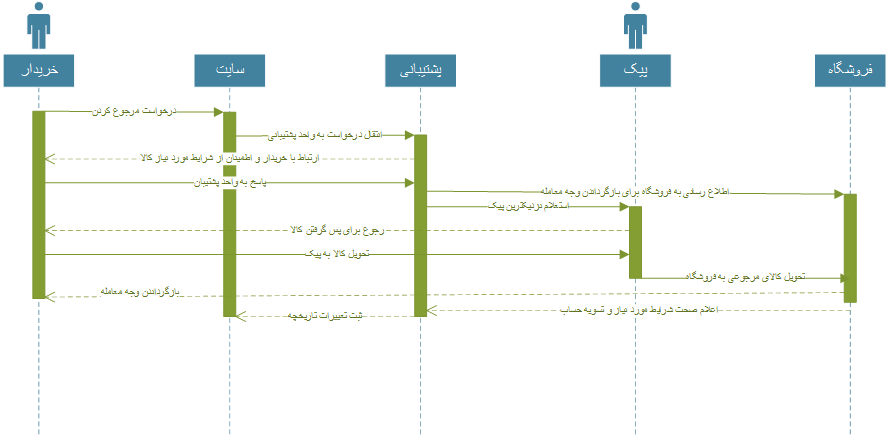
\includegraphics[width=14cm]{Sequence_Diagram_return}}
\caption{نمودار توالی فرآیند مرجوع کردن کالا}\label{figpvb}
\end{figure}




\end{document}